% ########### FILL THESE IN #############
% #######################################
\def\mytitle{Design of 4-BIT comparator}
\def\mykeywords{}
\def\myauthor{Mukesh chinta }
\def\contact{mukeshchinta1313@gmail.com}
\def\mymodule{Future Wireless Communication(FWC22069)}
% #######################################
% #### YOU DON'T NEED TO TOUCH BELOW ####
% #######################################
\documentclass[10pt, a4paper]{article}
\usepackage[a4paper,outer=1.5cm,inner=1.5cm,top=1.75cm,bottom=1.5cm]{geometry}
\twocolumn
\usepackage{graphicx}
\usepackage{circuitikz}
\usetikzlibrary{calc}
\graphicspath{{./images/}}
%colour our links, remove weird boxes
\usepackage[colorlinks,linkcolor={black},citecolor={blue!80!black},urlcolor={blue!80!black}]{hyperref}
\usetikzlibrary{arrows,shapes.gates.logic.US,shapes.gates.logic.IEC,calc}
%Stop indentation on new paragraphs
\usepackage[parfill]{parskip}
%% Arial-like font
\usepackage{lmodern}
\renewcommand*\familydefault{\sfdefault}
%Napier logo top right
\usepackage{watermark}
%Lorem Ipusm dolor please don't leave any in you final report ;)
\usepackage{lipsum}
\usepackage{xcolor}
\usepackage{listings}
%give us the Capital H that we all know and love
\usepackage{float}
%tone down the line spacing after section titles
\usepackage{titlesec}
%Cool maths printing
\usepackage{amsmath}
%PseudoCode
\usepackage{algorithm2e}
\usepackage{circuitikz}

\titlespacing{\subsection}{0pt}{\parskip}{-3pt}
\titlespacing{\subsubsection}{0pt}{\parskip}{-\parskip}
\titlespacing{\paragraph}{0pt}{\parskip}{\parskip}
\newcommand{\figuremacro}[5]{
    \begin{figure}[#1]
        \centering
        \includegraphics[width=#5\columnwidth]{#2}
        \caption[#3]{\textbf{#3}#4}
        \label{figure:#2}
    \end{figure}
}

\lstset{
frame=single, 
breaklines=true,
columns=fullflexible
}

\thiswatermark{\centering \put(0,-90.0){
\includegraphics[scale=0.05]{iith logo.png}} }
\title{\mytitle}
\author{\myauthor\hspace{1em}\\\contact\\IITH\hspace{0.5em}-\hspace{0.5em}\mymodule}
\date{}
\hypersetup{pdfauthor=\myauthor,pdftitle=\mytitle,pdfkeywords=\mykeywords}
\sloppy
% #######################################
% ########### START FROM HERE ###########
% #######################################
\usepackage{tabularx}
\begin{document}
	\maketitle
	\tableofcontents
	\begin{abstract}
	    %Replace the lipsum command with actual text 
Design a sequential circuit that take(A3,A2,A1,A0) and (B3,B2,B1,B0) compares both A and B.The o/p should  be either one of the (A<B),(A>B),(A=B) and it will be displayed by LED's.

	\end{abstract}
    \section{Introduction}
    A comparator is an electronic circuit, which compares the two 4-bit inputs that are applied to it and produces an output. The output value of the comparator indicates which of the inputs is greater,lesser or equal.
	\section{Components}
	
\begin{table}[htbp]
 \begin{center}
    \begin{tabular}{|l|c|c|c|c|c|c} \hline \textbf{Component}
  & \textbf{value} & \textbf{quantity} \\
 \hline
LED & 5V & 1 \\ \hline
Arduino & UNO & 1 \\ \hline
Jumper wires & M-M & 20\\ \hline

Bread board &  & 1 \\ \hline
\end{tabular}   
\end{center}
\caption{\label{table:table} }
\end{table}
	\section{Hardware}
    \begin{center}
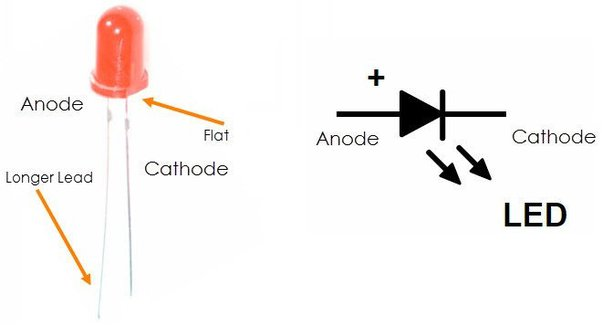
\includegraphics[scale=.20]{led.jpeg}
\end{center}
Figure 1: LED.
	\begin{table}[htbp]
    \begin{center}
    \begin{tabular}{|l|c|c|c|c|c|c|c|c|c|c|c|c} \hline \textbf{arduino}
  & 2 & 3 & 4 & 5 & 6 & 7 & 8 & 9 & 10 & 11 & 12 \\
 \hline
 \textbf{input} & a & b & c & d & e & f & g & h & & &  \\ \hline
\textbf{output} & & & & & & & &  & x & y & z \\ \hline
\end{tabular}   
\end{center}
\caption{\label{table:dummytable} }
\end{table}
\\	\textbf{3.2}
	connection of pins to the Arduino according to Table 2 and connecting VCC,GND of jumper wires to 5V,GND of Arduino respectively.
\\ \textbf{3.3}
Finally, give connections to the arduino and inputs based on table 3.
	\begin{table}[htbp]
    \begin{center}
    \begin{tabular}{|l|c|c|c|c|c|c|c|c|c|} \hline 
 
\textbf{Input} & a & b & c & d & e & f & g & h  \\ \hline
\textbf{Arduino} & 2 & 3 & 4 & 5& 6 & 7 & 8 & 9\\ \hline
\end{tabular}   
\end{center}
\caption{\label{table:dummytable} }
\end{table}
\section{Implementation}
\textbf{4.1}
By making Logic circuit based on 4-bit comparator logic we get the circuit as in figure 2.

\textbf{4.2}
The code below realizes the 4-bit comparator.
\begin{lstlisting}
https://github.com/mukeshchinta/FWC_module1/blob/main/assembly%20assignment/assemble/codes/4bit%20assembly.txt
\end{lstlisting}



 \begin{center}
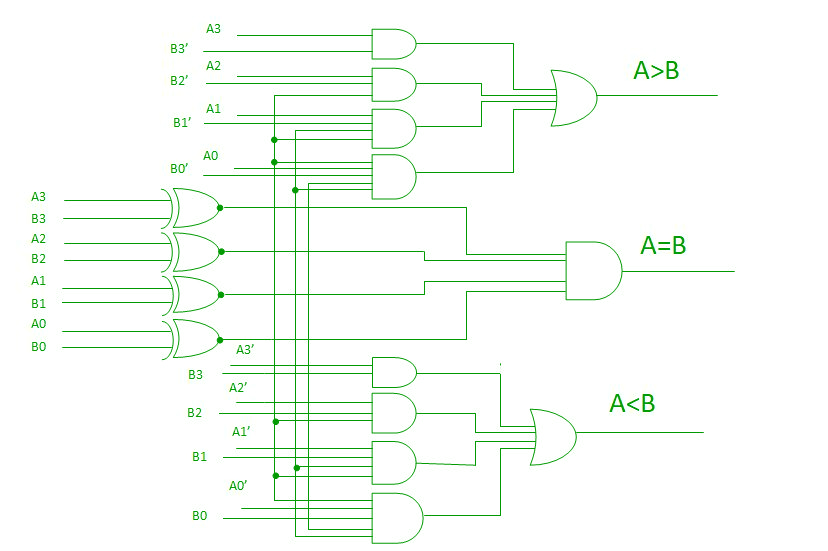
\includegraphics[scale=.40]{4bit.jpg}

\end{center}
\begin{center}
    Figure 2
\end{center}

\end{document}